\section{Problem 3}

\subsection{Part1}

{\bfseries Algorithm} \\
We first create a centered x data matrix Z. And then we cerate a centered y values.

\begin{equation}
z^{(i)}_{j} = x^{(i)}_{j} - \bar{x}_{j} \hspace{10 mm} 
y^{(i)}_{c} = y^{(i)} - \bar{y} \\
\end{equation}

Then we use the formula for calculating the error. It uses a $\lambda$ for regularizing the
weight terms. 

\begin{equation}
  E(w)= (Y_{c} - ZW)^T(Y_{c}-ZW) + \lambda W^TW \\
\end{equation}

We used a regularized term to calculate optimal weight using the following equation

\begin{equation}
  W_{ridge} = (Z^{T}Z + \lambda I)^{-1}Z^{T}Y_{c}
\end{equation}

{\bfseries Experimentation} \\
We have conducted a series of experimentation with the simple data from Bishop's Figure 1.4

%TODO: generate graphs to show the impact of increasing M (overfitting), but this is shown in the previou squestion
As M increases, the curve is more likely to overfit the data. 

We have conducted a series of experiments using M =1, M = 3 and M = 9 with varying lambdas. 


\begin{figure}[!htb]
\minipage{0.5\textwidth}
  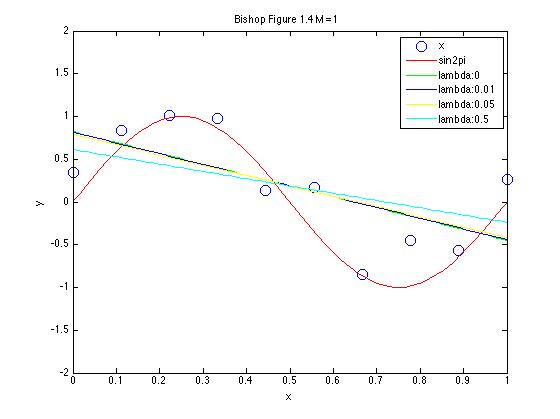
\includegraphics[width=\linewidth]{figures/p3_bishop_m=1}
  \caption{M = 1}\label{fig:figures/p3_bishop_m=1}
\endminipage\hfill
\minipage{0.5\textwidth}
  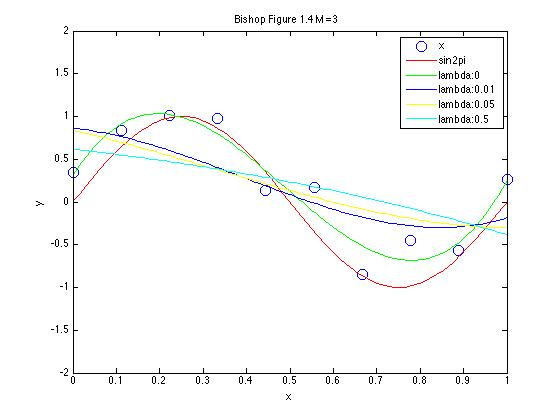
\includegraphics[width=\linewidth]{figures/p3_bishop_m=3}
  \caption{M = 3}\label{fig:figures/p3_bishop_m=3}
\endminipage\hfill
\minipage{0.5\textwidth}%
  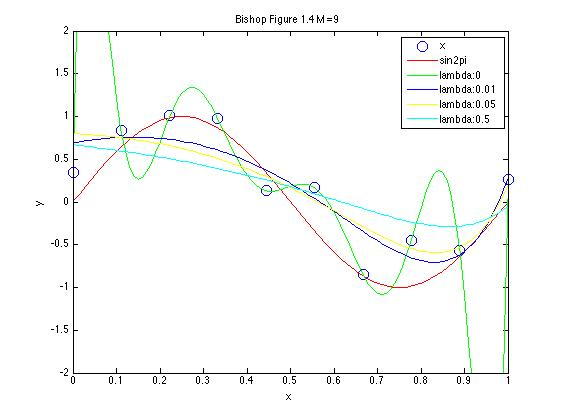
\includegraphics[width=\linewidth]{figures/p3_bishop_m=9}
  \caption{M = 9}\label{fig:figures/p3_bishop_m=9}
\endminipage
\end{figure}



%% \begin{figure}[h]

%%   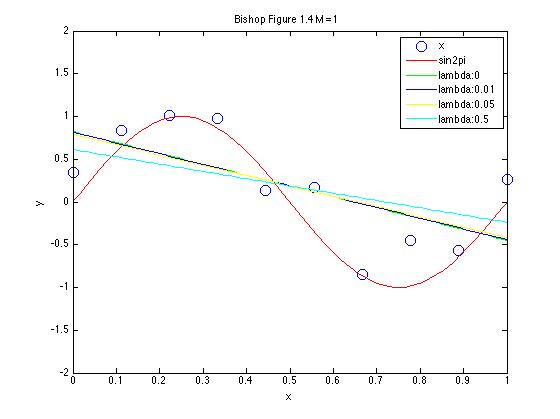
\includegraphics[width=0.5\textwidth]{figures/p3_bishop_m=1}
%%   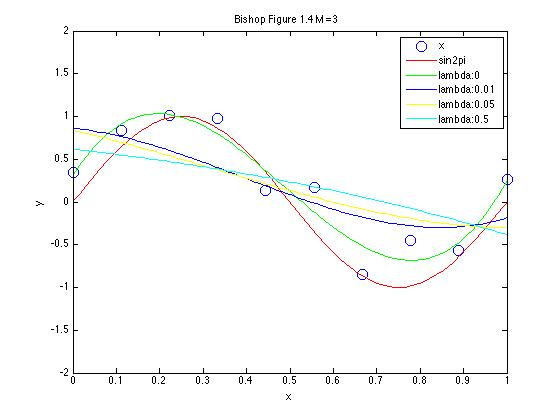
\includegraphics[width=0.5\textwidth]{figures/p3_bishop_m=3}
%%   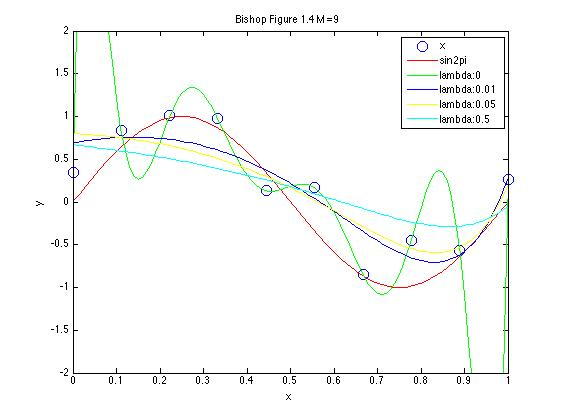
\includegraphics[width=0.5\textwidth]{figures/p3_bishop_m=9}

%% \end{figure}

we can see that for a smaller M, changing the lambda doesn't impact the performance as much. It bends the graph in the more general direction. For a large M, the lambda greatly reduces the overfitting problem. As a result, even with a large M, the model can be more generalized. 

\subsection{Part2}


%TODO: generate graphs to show the impact of increasing M (overfitting)

%TODO: generate graphs to show the inmpact of increaing lambda

%TODO: show that the models trained from data A is a lot better than model B

First, we can see that in general error from training set B is higher than that from training set A. 
This is because there is a outlier in trainng set B. This prevented us from creating a good model. 



\begin{figure}[!htb]
\minipage{0.32\textwidth}
  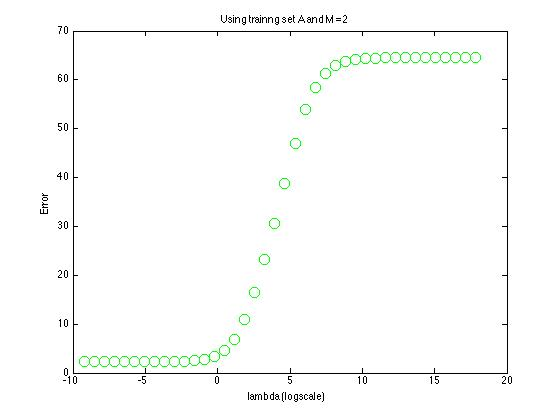
\includegraphics[width=\linewidth]{figures/p3_regressA_m=2}
  \caption{M = 2}\label{fig:figures/p3_regressA_m=2}
\endminipage\hfill
\minipage{0.32\textwidth}
  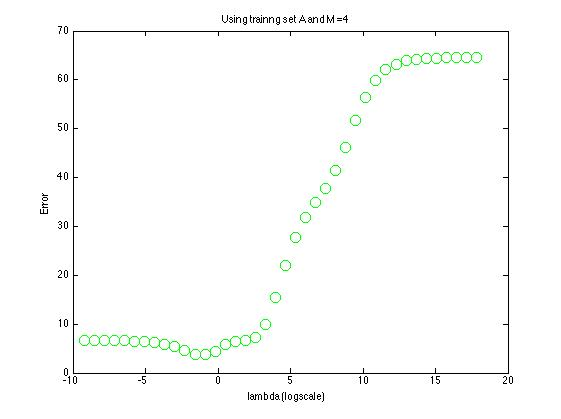
\includegraphics[width=\linewidth]{figures/p3_regressA_m=4}
  \caption{M = 4}\label{fig:figures/p3_regressA_m=4}
\endminipage\hfill
\minipage{0.32\textwidth}%
  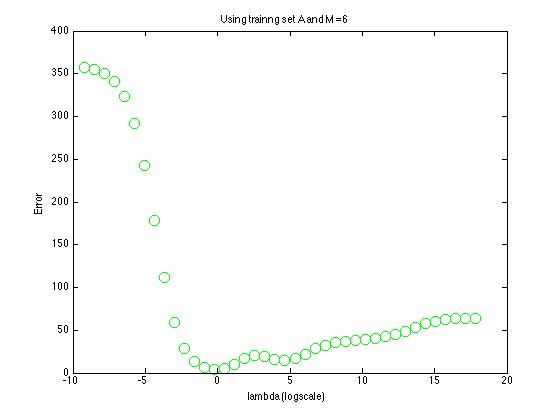
\includegraphics[width=\linewidth]{figures/p3_regressA_m=6}
  \caption{M = 6}\label{fig:figures/p3_regressA_m=6}
\endminipage
\end{figure}


\begin{figure}[!htb]
\minipage{0.32\textwidth}
  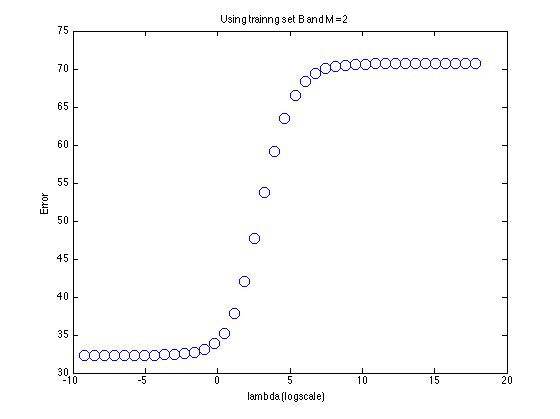
\includegraphics[width=\linewidth]{figures/p3_regressB_m=2}
  \caption{M = 2}\label{fig:figures/p3_regressB_m=2}
\endminipage\hfill
\minipage{0.32\textwidth}
  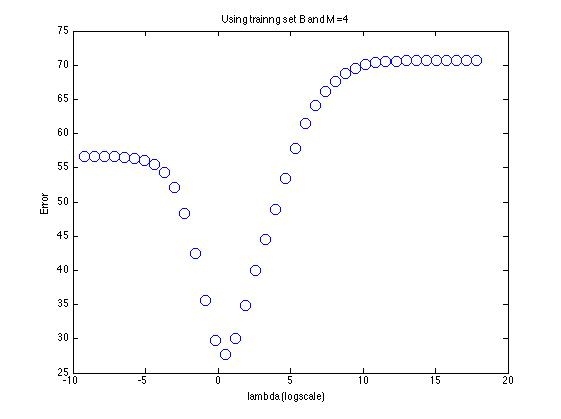
\includegraphics[width=\linewidth]{figures/p3_regressB_m=4}
  \caption{M = 4}\label{fig:figures/p3_regressB_m=4}
\endminipage\hfill
\minipage{0.32\textwidth}%
  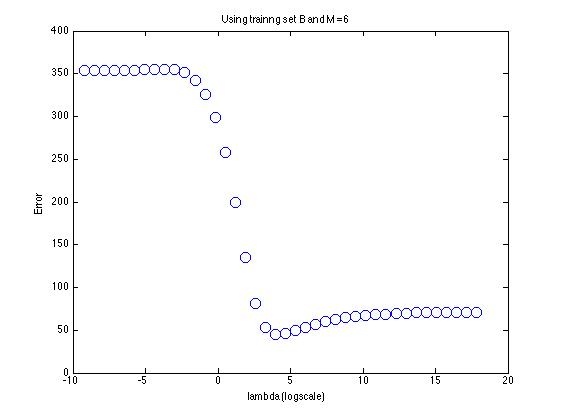
\includegraphics[width=\linewidth]{figures/p3_regressB_m=6}
  \caption{M = 6}\label{fig:figures/p3_regressB_m=6}
\endminipage
\end{figure}


\subsection{Part3}
